\documentclass[final]{beamer}
\usepackage{hyperref,xspace,graphicx,microtype,minted,multicol,mflogo,enumerate,mathtools,hologo}
\usepackage[brazil]{babel}

\usetheme[sectionpage=simple,numbering=none]{metropolis}
\beamertemplatenavigationsymbolsempty

\newcommand{\filename}[1]{\texttt{#1}}
\newcommand{\code}[1]{\texttt{#1}}

\title{Introdução ao \LaTeX}
\author{Rafael Beraldo}
% Seções:
% 1. 28 de maio de 2016
% 2. 25 de julho de 2016
\date{25 de julho de 2016}

\begin{document}
\maketitle
% TODO: add kind of table of contents
% História %%%%%%%%%%%%%
\begin{frame}[standout]
  \Huge História
\end{frame}

\begin{frame}[plain]
  \begin{figure}[h]
    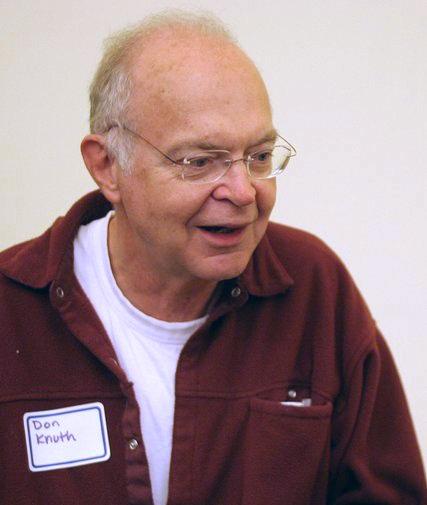
\includegraphics[scale=.5]{imagens/knuth}
    \caption{Donald Knuth em 2005}
  \end{figure}
\end{frame}

\begin{frame}[plain]
  \hspace*{-11.5mm}
  \begin{centering}
    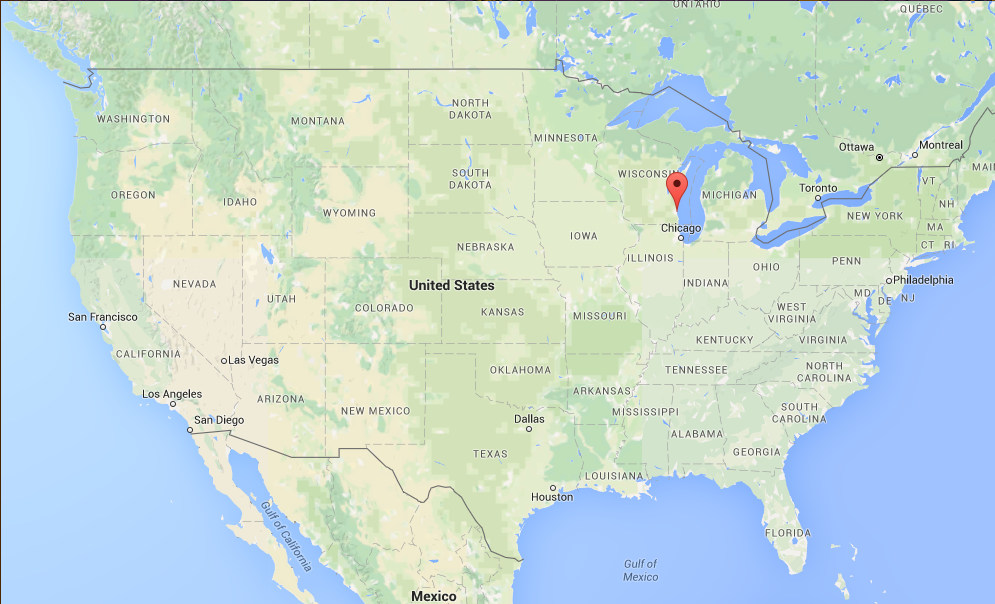
\includegraphics[width=\pagewidth]{imagens/milwaukee}
  \end{centering}
\end{frame}

\begin{frame}
  \Huge
  \only<1>{O pai de Knuth tinha uma editora}
  \only<2>{1977: segunda edição do segundo volume de \emph{The Art of Computer
  Programming}}
  \only<3>{\textsc{ascii} não foi projetado com livros em mente}
  \only<4>{\TeX: tau epsilon chi}
\end{frame}

\begin{frame}
  \large
  \begin{quote}
    The purpose of this pronunciation exercise is to remind you that \TeX\ is
    primarily concerned with high-quality technical manuscripts: Its emphasis
    is on art and technology, as in the underlying Greek word. If you merely
    want to produce a passably good document—something acceptable and basically
    readable but not really beautiful—a simpler system will usually suffice.
    With \TeX\ the goal is to produce the finest quality; this requires more
    attention to detail, but you will not find it much harder to go the extra
    distance, and you’ll be able to take special pride in the finished
    product.\hfill (Donald Knuth, \emph{\TeX book})
  \end{quote}
\end{frame}

\begin{frame}
  \Huge
  \LaTeX: 1985
\end{frame}

\begin{frame}[plain]
  \begin{figure}[h]
    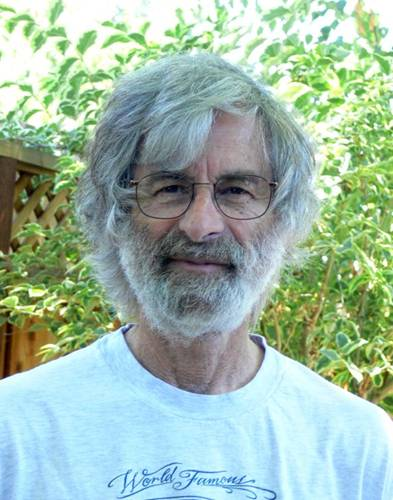
\includegraphics[scale=.5]{imagens/lamport}
    \caption{Leslie Lamport}
  \end{figure}
\end{frame}

% Filosofia %%%%%%%%%%%%%
\begin{frame}[standout]
  \Huge Filosofia
\end{frame}

% Considerações iniciais
\begin{frame}
  \only<1>{\Huge\LaTeX{} é uma linguagem de marcação de texto}
  \only<2>{\Huge Você \emph{declara} o documento}
  \only<3>{\Huge É como um tipógrafo profissional à sua disposição}
  \only<4>{\Huge Assim como em \textsc{html}, o arquivo fonte é renderizado}
  \only<5>{\Huge Comandos são semânticos}
\end{frame}

% Sintaxe dos comandos
\begin{frame}[fragile]
  \begin{minted}[autogobble,fontsize=\huge,breaklines]{latex}
    \section{Introdução}
  \end{minted}
\end{frame}

%
% hello-world.tex
%
% Rafael Beraldo <rberaldo@cabaladada.org>
% Workshop de LaTeX do Opensanca
% 28 de maio de 2016
% 
% Demonstra:
% - Estrutura do documento
% - Compilação
% - Comandos (\section, \LaTeX)
% - Classes (article, minimal) e suas opções
%

\documentclass{article}
\begin{document}
Hello, world!
\end{document}

%
% simbolos-reservados.tex
%
% Rafael Beraldo <rberaldo@cabaladada.org>
% Workshop de LaTeX do Opensanca
%
% Problema: o arquivo a seguir não irá compilar corretamente, pois usa símbolos
% reservados ao LaTeX. Corrija os problemas até que a compilação seja
% bem-sucedida.
%

\documentclass{article}
\begin{document}
Nossos teclados são bem limitados em termos de símbolos. Provavelmente por
isso, os poucos símbolos que temos à nossa disposição foram tomando sentidos
diferentes com o passar do tempo.

É muito comum, por exemplo, substituir a letra “e” pelo &. Em alguns contextos
na Internet, a # é usada para indicar tags. Em alguns casos, _underlines_ são
equivalentes a um texto itálico. E no \LaTeX, o símbolo \ indica o começo de um
comando.
\end{document}

%
% espaco-branco.tex
%
% Rafael Beraldo <rberaldo@cabaladada.org>
% Workshop de LaTeX do Opensanca
% 28 de maio de 2016
% 
% Demonstra:
% - Tratamento de espaços em branco
% - Novas linhas e parágrafos
%

\documentclass{minimal}
\begin{document}
  Muito       além, nos confins     inexplorados da região mais     brega da Borda Ocidental desta Galáxia, há um pequeno sol amarelo e esquecido.
  Girando em torno deste sol, a uma distância de cerca de 148 milhões de quilômetros, há um planetinha verde-azulado absolutamente insignificante.
\end{document}

% poliglota-exercicio.tex %%%%%%%%%%%%%%
\begin{frame}[standout]
  \huge
  \filename{poliglota-exercicio.tex}
\end{frame}

% No exemplo anterior, espaco-branco.tex, os acentos — na verdade, diacríticos
% — não apareceram. Alguém saberia o motivo?
\begin{frame}
  \frametitle{\filename{poliglota-exercicio.tex}}
  \huge
  Acentos não apareciam em \filename{espaco-branco.tex}
\end{frame}

% Para resolver, teremos que usar pacotes
\begin{frame}
  \frametitle{\filename{poliglota-exercicio.tex}}
  \Huge
  Solução: pacotes
\end{frame}

% Para carregar pacotes, usamos esta sintaxe
\begin{frame}[fragile]
  \frametitle{\filename{poliglota-exercicio.tex}}
  \begin{minted}[autogobble,fontsize=\LARGE,breaklines]{latex}
    \usepackage[opções]{pacote}
  \end{minted}
\end{frame}

% Para resolvermos a falta de diacríticos, usaremos o pacote polyglossia
\begin{frame}
  \frametitle{\filename{poliglota-exercicio.tex}}
  \Huge
  Pacote \code{polyglossia}
\end{frame}

\begin{frame}
  \frametitle{\filename{poliglota-exercicio.tex}}
  \Huge
  O \code{polyglossia} traz benefícios como:
  \begin{itemize}
    \only<1>{\item Hifenização}
    \only<2>{\item Strings como \mintinline{latex}{\today}}
    \only<3>{\item Convenções tipográficas localizadas}
  \end{itemize}
\end{frame}

% Ao exercício.
%
% Sabemos para que serve o polyglossia. Perguntar como ele seria implementado,
% e onde seria colocado no código.
%
% Também estudar a sintaxe para selecionar línguas. Explicar o motivo pelo qual
% a opção de pacote [brazil] não é mais usada: fica difícil selecionar várias
% línguas e suas opções.
\begin{frame}
  \frametitle{\filename{poliglota-exercicio.tex}}
  \Huge
  Como carregar o pacote \code{polyglossia}?
\end{frame}

\begin{frame}[fragile]
  \frametitle{\filename{poliglota-exercicio.tex}}
  \begin{minted}[autogobble,fontsize=\Large,breaklines]{latex}
    \usepackage{polyglossia}
    \setdefaultlanguage{brazil}
  \end{minted}
\end{frame}

% Para encontrar ajuda, podemos ler a documentação oficial dos pacotes que
% estamos usando. Mostrar outras opções do polyglossia, por exemplo.
\begin{frame}
  \frametitle{\filename{poliglota-exercicio.tex}}
  \Huge
  Comprehensive \TeX{} Archive Network

  \url{www.ctan.org}
\end{frame}

\begin{frame}
  \frametitle{\filename{poliglota-exercicio.tex}}
  \huge
  \url{www.ctan.org/pkg/polyglossia}
\end{frame}

%
% artigo-exemplo.tex
%
% Rafael Beraldo <rberaldo@cabaladada.org>
% Workshop de LaTeX do Opensanca
% 28 de maio de 2016
% 
% Demonstra:
% - Organização de um documento LaTeX
% - Opções das classes
% - Efeitos da mudança de classe
% - Mais pacotes: blindtext, hyperref e microtype
% - Como inserir links
%

\documentclass[11pt,a4paper,oneside]{article}
\usepackage{polyglossia}
  \setdefaultlanguage{brazil}
\usepackage{blindtext,hyperref}

\title{Meu artigo muito sério e importante}
\author{Rafael Beraldo}

\begin{document}
\frenchspacing

\maketitle

\begin{abstract}
  \blindtext
\end{abstract}

\tableofcontents

\section{Introdução}
\blindtext

\section{Metodologia}
\blindtext

\section{Conclusão}
\blindtext

\end{document}

%
% fontes.tex
%
% Rafael Beraldo <rberaldo@cabaladada.org>
% Workshop de LaTeX do Opensanca
% 28 de maio de 2016
% 
% Demonstra:
% - Codificação de fontes e de input: OT1, T1 e TU
% - Demonstrar os efeitos usar essas codificações, inclusive para copiar textos
% - Inserção de diacríticos antes e hoje
% - Tamanhos e estilos de fonte
% - Como selecionar outras fontes
%

\documentclass[11pt,a4paper,oneside]{article}
% Codificação padrão do LaTeX, conhecida como OT1 (Old Text 1):
% \usepackage[OT1]{fontenc}
%
% Codificação mais recente, T1 (Text 1), com suporte para muitas línguas
% europeias. Podemos inserir caracteres em Unicode:
% \usepackage[T1]{fontenc}
% \usepackage[utf8]{inputenc}
%
% O pacote fontspec usa a codificação TU (TeX Unicode) por padrão:
\usepackage{fontspec}
% Selecionar fontes:
% \setmainfont{Linux Libertine}
%
% Selecionar a língua:
\usepackage{polyglossia}
  \setdefaultlanguage{brazil}
\usepackage{microtype}

\title{Fontes no \LaTeX}
\author{Rafael Beraldo}

\begin{document}
\frenchspacing

\maketitle

\section{Codificações}

Este é um parágrafo cheio de acentos e palavras. Antigamente, seria necessário
escrever “tip\'{o}grafos trabalhar\~{a}o”, mas hoje é fácil adicionar símbolos
Unicode diretamente, como esta seta: →

\section{Fontes e suas famílias} 

No passado, fontes não costumavam ter \emph{tantos} estilos. Tipógrafos
compunham livros inteiros com apenas um tipo e um tamanho. Hoje, temos uma
miríade de possibilidades. Empregá-las com sabedoria e, talvez, um pouco de
parcimônia não são más ideias.

As fontes que usamos comumente contam com tipos como:

\begin{itemize}
  \item O \emph{itálico,} geralmente usado para enfatizar ideias.
  \item O \textbf{negrito}, ou \textbf{bold}, muitas vezes usado para chamar a
    atenção do leitor.
  \item Os \textsc{versaletes}, que são letras em estilo de maiúscula, mas com
    a mesma altura do corpo da fonte. Uma boa ideia é usá-los em siglas, como
    \textsc{ibge}, \textsc{bc}, 3~\textsc{am} etc. Em nomes próprios e
    acrônimos geográficos, geralmente usamos maiúsculas como JRR Tolkien.
  \item Os \texttt{tipos monoespaçados} são ótimos para dar exemplos de
    código-fonte ou nomes de arquivos, como \texttt{fontes.tex}.
\end{itemize}

\section{Tamanhos de fontes}

Como já vimos, certos comandos como \verb+\section+ e \verb+chapter+ escolhem o
tamanho e espaçamento adequados para que nosso texto pareça organizado e
fluido. Essas decisões são tomadas pelos designers das classes que usamos e
baseadas em \textbf{escalas} tipográficas. Nas raras ocasiões em que precisamos
\footnotesize diminuir \Large ou aumentar \normalsize nosso texto, temos os seguintes
comandos à nossa disposição:

\begin{itemize}
  \item\verb+\tiny+
  \item\verb+\scriptsize+
  \item\verb+\footnotesize+
  \item\verb+\small+
  \item\verb+\normalsize+
  \item\verb+\large+
  \item\verb+\Large+
  \item\verb+\LARGE+
  \item\verb+\huge+
  \item\verb+\Huge+
\end{itemize}

{\Large É possível conter nosso texto entre duas chaves} para que apenas uma
seção seja afetada pelo comando de tamanho.

\end{document}

% layouts-pagina.tex %%%%%%%%%%%%%%
\begin{frame}[standout]
  \Huge
   \filename{layouts-pagina.tex}
\end{frame}

% Vamos mudar a opção de classe de onecolumn para twocolumn e carregar o pacote
% showframe.
\begin{frame}
  \frametitle{\filename{layouts-pagina.tex}}
  \huge
  \only<1>{Copiar solução de \filename{fontes-exercio.tex} em
  \filename{layouts-pagina.tex}}
  \only<2>{Mudar para \code{twocolumn}, carregar o pacote \code{showframe}}
\end{frame}

% Na folha A4, apenas uma coluna coluna de texto é difícil de ler com margens
% curtas. Mas usar margens grandes desperdiça papel.
\begin{frame}
  \frametitle{\filename{layouts-pagina.tex}}
  \huge
  \code{onecolumn}: margens grandes demais

  \code{twocolumn}: nem sempre podemos
\end{frame}

% Soluções para o problema do tamanho da coluna de texto vs margens
\begin{frame}
  \frametitle{\filename{layouts-pagina.tex}}
  \huge
  Soluções:
  \begin{itemize}
    \only<1>{\item Colunas}
    \only<2>{\item \code{fullpage}}
    \only<3>{\item \code{fullpage} e entrelinhas maiores}
  \end{itemize}
\end{frame}

% Se decidirmos usar o pacote fullpage, é uma boa ideia aumentar o espaçamento
% entre as linhas.
\begin{frame}
  \frametitle{\filename{layouts-pagina.tex}}
  \huge
  Pacote \code{setspace}:

  \begin{itemize}
    \item \code{\textbackslash singlespacing}
    \item \code{\textbackslash onehalfspacing}
    \item \code{\textbackslash doublespacing}
  \end{itemize}
\end{frame}

% Outro fator que influencia o layout da página é seu estilo. Estes são os três
% comandos básicos e estilos que podemos escolher.
\begin{frame}
  \frametitle{\filename{layouts-pagina.tex}}
  \huge
  \code{\textbackslash pagestyle} e \code{\textbackslash thispagestyle}

  \begin{itemize}
    \item \code{empty}
    \item \code{plain}
    \item \code{headings}
  \end{itemize}
\end{frame}

% Outro fator que influencia o layout da página é seu estilo. Estes são os três
% comandos básicos e estilos que podemos escolher.
\begin{frame}
  \frametitle{\filename{layouts-pagina.tex}}
  \huge
  Demonstração em \filename{layouts-pagina.tex}
\end{frame}

% Exercício: faremos um certificado de conclusão do curso
\begin{frame}
  \frametitle{\filename{layouts-pagina-exercicio.tex}}
  \Huge
  Certificado de conclusão
\end{frame}

% Uma certificado incompleto
\begin{frame}[plain]

  {\huge\textbf{OpenSanca}}\\[2em]
  {\LARGE\textsc{Certificado}}

  \noindent Certificamos que Tal Pessoa da Silva participou de um curso em
  nosso grupo no dia 28 de maio de 2016 e está qualificado para editar textos
  em \LaTeX.

  \vfill
  \emph{Os Organizadores}\\
  \emph{OpenSanca}

\end{frame}

% Começar nosso certificado de conclusão de curso
\begin{frame}
  \frametitle{\filename{layouts-pagina.tex}}
  \Huge
  Resolver \filename{layouts-pagina-exercicio.tex}
\end{frame}

%
% posicao-texto.tex
%
% Rafael Beraldo <rberaldo@cabaladada.org>
% Workshop de LaTeX do Opensanca
%
% Demonstra:
% - Ambientes center, flushleft e flushright
% - Como controlar o espaço horizontal e vertical com \hspace, \vspace, \hfill
%   e \vfill
% - Diferentes unidades que o LaTeX conhece
%

\documentclass[a4paper,oneside]{article}
\usepackage{fontspec}
\usepackage{polyglossia}
  \setdefaultlanguage{brazil}

\begin{document}
\frenchspacing

\section{Ambientes}

Para posicionar o texto horizontalmente na página, podemos usar três
\textbf{ambientes}: \texttt{center, flushleft} e \texttt{flushright}.

\begin{center}
  Todo este texto será centralizado na página.
\end{center}

\begin{flushleft}
  Esse parágrafo será alinhado à esquerda e não será justificado. Mais abaixo,
  veremos como ajustar a posição de um texto dentro da própria linha.
\end{flushleft}

\begin{flushright}
  Também podemos alinhar texto à direita. Além desses ambientes, podemos mudar
  o alinhamento do texto usando os comandos \verb+\centering+,
  \verb+\flushleft+ e \verb+\flushright+.
\end{flushright}

\section{Controlando o espaço na linha}

Os comandos \verb+\hspace{comprimento}+ e \verb+\hfill+ nos permitem controlar
o espaço dentro de uma linha:

Aqui haverá\hspace{1.5cm} um espaço.

Começo\hfill meio\hfill fim.

\section{Espaço vertical}

Os comandos para controle do espaço vertical, isto é, o espaço entre os
parágrafos, são muito parecidos com os comandos de espaço horizontal. Eles são
\verb+\vspace{comprimento}+ e \verb+\vfill+.
\end{document}

% listas.tex %%%%%%%%%%%%%%
\begin{frame}[standout]
  \Huge
  \filename{listas.tex}
\end{frame}

% Três tipos de listas inclusos por padrão
\begin{frame}
  \frametitle{\filename{listas.tex}}
  \Huge
  Ambientes: \code{itemize, enumerate} e \code{description}
\end{frame}

% Anatomia de uma lista
\begin{frame}[fragile]
  \frametitle{\filename{listas.tex}}
  \LARGE
  Ingredientes para carbonara:

  \begin{minted}[autogobble,fontsize=\Large,breaklines]{latex}
    \begin{itemize}
      \item Bacon
      \item Macarrão
      \item Ovos
      \item Parmesão
      \item Pimenta-do-reino
    \end{itemize}
  \end{minted}
\end{frame}

% Existem mais listas no arquivo listas.tex
\begin{frame}
  \frametitle{\filename{listas.tex}}
  \Huge
  Aprenderemos mais em \filename{listas.tex}
\end{frame}

% Exercício: completar a receita de panqueca com os ingredientes corretos.
\begin{frame}
  \frametitle{\filename{listas.tex}}
  \Huge
  Resolver \filename{listas-exercicio.tex}
\end{frame}

% Lista de ingredientes que os participantes devem colocar na receita. Notar a
% palavra ingrediente, o número sequencial e o parênteses.
\begin{frame}
  \frametitle{\filename{listas.tex}}
  \large
  \begin{enumerate}[{Ingrediente} 1)]
    \item 190g de farinha
    \item 25g de açúcar
    \item 10g de fermento químico em pó
    \item 3g de sal\\[1em] … texto …\\
    \item 25g de manteiga\\[1em] … texto …\\
    \item 330g de leite
    \item 80g de ovos
  \end{enumerate}
\end{frame}

% citacoes-versos.tex %%%%%%%%%%%%%%
\begin{frame}[standout]
  \Huge
  \filename{citacoes-versos.tex}
\end{frame}

% Ambientes quote e quotation
\begin{frame}
  \frametitle{\filename{citacoes-versos.tex}}
  \Huge
  Ambientes: \code{quote} e \code{quotation}
\end{frame}

% Exemplo de uso do ambiente quote
\begin{frame}[fragile]
  \frametitle{\filename{citacoes-versos.tex}}
  \Large
  \begin{minted}[autogobble,fontsize=\Large,breaklines]{latex}
  \begin{quote}
    Não entre em pânico!\hfill (Douglas Adams)
  \end{quote}
  \end{minted}
  \vspace{1em}

  \begin{quote}
    Não entre em pânico!\hfill (Douglas Adams)
  \end{quote}
\end{frame}

% Exemplo de uso do ambiente verse
\begin{frame}[fragile]
  \frametitle{\filename{citacoes-versos.tex}}
  \begin{minted}[autogobble,fontsize=\large,breaklines]{latex}
    \begin{verse}
      O vinho dá-te o calor que não tens;\\
      suaviza o jugo do passado e te alivia\\
      das brumas do futuro; inunda-te de luz\\
      e te liberta desta prisão.
      \flushright
      (Omar Khayyam)
    \end{verse}
  \end{minted}
\end{frame}

% Output do comando anterior
\begin{frame}
  \frametitle{\filename{citacoes-versos.tex}}
  \Large
  \begin{verse}
    O vinho dá-te o calor que não tens;\\
    suaviza o jugo do passado e te alivia\\
    das brumas do futuro; inunda-te de luz\\
    e te liberta desta prisão.
    \flushright
    (Omar Khayyam)
  \end{verse}
\end{frame}

%
% tabelas.tex % % Rafael Beraldo <rberaldo@cabaladada.org>
% Workshop de LaTeX do Opensanca
%
% Demonstra:
% - O ambiente tabular
% - Como implementar tabelas usando mais espaço em branco ao invés de linhas
% - Como colocar parágrafos dentro de células
% - O pacote booktabs
% - Células com várias colunas usando \multicolumn
% - O pacote longtable
% - Floats e o ambiente table
%

\documentclass[a4paper,oneside]{article}
\usepackage{fontspec}
\usepackage{polyglossia}
  \setdefaultlanguage{brazil}

\begin{document}
\frenchspacing

\section{Uma tabela básica}

Usando a tabela abaixo, vamos aprender como alinhar texto dentro das células de
um ambiente \texttt{tabular}:

\begin{center}
  \begin{tabular}{l c r}
    1 & 2 & 3\\
    4 & 5 & 6\\
    7 & 8 & 9\\
  \end{tabular}
\end{center}

% A seção a seguir foi inspirada no site
% http://www.thefreshloaf.com/lessons/yourfirstloaf
\section{Ingredientes básicos para o pão}

Apenas quatro ingredientes são necessários para fazer pão. Vejamos uma receita
genérica:

% Brincar com as possibilidades aqui
\begin{center}
  \begin{tabular}{lr}
    Ingrediente & Quantidade\\[5pt]
    Trigo    & 3 xíc\\
    Sal      & 2 cc\\
    Fermento & 2 cc\\
    Água     & 1 $^1/_7$ xíc
  \end{tabular}
\end{center}

Antes de correr para a cozinha, é fundamental entender para que servem e como
interagem esses ingredientes.

% Trocar o tamanho do parágrafo
\begin{center}
  \begin{tabular}{lp{.6\textwidth}}
      Ingrediente & Função\\[5pt]
      Trigo       & A base do pão. Sem trigo, sem pão.\\
      Sal         & Retarda o fermento e controla o processo de fermentação.
                      Também adiciona o sabor que todo esperamos do pão.\\
      Fermento    & É comumente vendido seco e precisa ser ativado com água
                      morna.  Faz o pão crescer e quanto maior a quantidade,
                      mais rápido é o crescimento. Fermento demais deixa o pão
                      com um gosto de cerveja.\\
      Água        & Dissolve os ingredientes (solvente universal, alguém?) e
                      ativa o fermento. Ao adicionar mais água, o resultado é
                      um pão mais pegajoso e com buracos menos regulares. Se
                      houver muito pouca água, a expansão da massa é restrita e
                      o resultado é um pão mais firme, seco e duro.
  \end{tabular}
\end{center}

Imprima o resumo abaixo e cole na parede da cozinha, para nunca esquecer esses
princípios básicos:

% É possível induzir quebras de linha explícitas dentro de um parágrafo em uma
% célula, se ela incluir o comando \raggedright ou \centering. Nesses casos,
% precisamos usar \tabularnewline para começar uma nova linha.
%
% Também introduzir o pacote booktabs, que nos permite usar os comandos
% \toprule, \midrule and \bottomrule. Discutir como, frequentemente, não são
% necessários para melhorar a legibilidade.
\begin{center}
  \begin{tabular}{lp{.6\textwidth}}
    Ingrediente & Função\tabularnewline[8pt]
    Trigo & Base do pão\tabularnewline[3pt]
    Sal & \raggedright Retarda o fermento\\
                    Controla o processo de fermentação\\
                    Dá sabor ao pão\tabularnewline[3pt]
    Fermento & \raggedright Vendido seco\\
                    Ativado com água morna\\
                    Faz o pão crescer\\
                    Em abundância, o crescimento é mais
                    rápido\tabularnewline[3pt]
    Água & \raggedright Dissolve os ingredientes\\
                    Ativa o fermento\\
                    Em abundância, pão mais pegajoso e com buracos menos
                    regulares\\
                    Em falta, pão mais firme, duro e seco
  \end{tabular}
\end{center}

% Informação encontrada em
% http://www.space.com/images/i/000/024/511/original/nearest-stars-121218g-02.jpg
\section{Distâncias cósmicas}

Com uma nave que viaje à velocidade da luz, seriam necessários 4,2 anos para
chegar à estrela mais próxima. Abaixo, uma lista de destinos para quem dispõe
de tempo livre.

% Estamos demonstrando dois conceitos aqui: como poderíamos usar um \midrule
% depois de multicolumn e, é claro, multicolumn. Vamos aproveitar para
% deixá-la mais longa e carregar o pacote longtable. O comando \endhead é útil
% para definir um cabeçalho que se repete em toda página.
\begin{center}
  \begin{tabular}{lr}
    \multicolumn{2}{c}{Estrelas na Via Láctea}\\[8pt]
    Estrela            & Distância (anos-luz)\\[5pt]
    Proxima Centauri   & 4,2\\
    Rigil Kentaurus    & 4,3\\
    Alpha Cen B        & 4,3\\
    Estrela de Barnard & 6,0\\
    Wolf 359           & 7,7\\
    BD +36 2147        & 8,2\\
    Luyten 726-8A      & 8,4\\
    Luyten 726-8B      & 8,4\\
    Sirius A           & 8,6\\
    Sirius B           & 8,6\\
    Ross 154           & 9,4\\
    Ross 248           & 10,4\\
    Epsilon Eri        & 10,8\\
    Ross 128           & 10,9\\
    61 Cyg A           & 11,1\\
    61 Cyg B           & 11,1\\
    Epsilon Ind        & 11,2\\
    BD +43 44 A        & 11,2\\
    BD +43 44 B        & 11,2\\
    Luyten 789-6       & 11,2\\
    Procyon A          & 11,4\\
    Procyon B          & 11,4\\
    BD +59 1915 A      & 11,6\\
    BD +59 1915 B      & 11,6\\
    CoD -36 15693      & 11,7
  \end{tabular}
\end{center}
\end{document}

%
% imagens.tex
%
% Rafael Beraldo <rberaldo@cabaladada.org>
% Workshop de LaTeX do Opensanca
% 28 de maio de 2016
%
% Demonstra:
% - Como incluir gráficos com o pacote graphicx
% - Controlar o tamanho e escala dos gráficos
% - O ambiente figure
% - O ambiente minipage e seus usos
%

\documentclass[a4paper,oneside]{article}
\usepackage{fontspec}
\usepackage{polyglossia}
  \setdefaultlanguage{brazil}
\usepackage{microtype,graphicx}

\begin{document}
\frenchspacing

% Informação e imagem encontrados na Wikipédia em:
% https://en.wikipedia.org/wiki/Alpha_Centauri
\section{Nosso vizinhos}

Na figura~\ref{fig:estrelas}, podemos ver nossos vizinhos mais próximos, por
assim dizer. A estrela circulada é Proxima Centauri, uma pequena anã vermelha,
que pode estar ligada gravitacionalmente às outras duas estrelas. A olho nu, as
duas estrelas parecem uma só.

% Brincar os as opções de posicionamento do figure e de tamanho do
% \includegraphics. Ensinar o ambiente minipage, e a técnica de colocar dois
% minipages dentro de um figure para colocar uma imagem ao lado da outra.
\begin{figure}[h]
  \centering
  \includegraphics[width=\textwidth]{estrelas}
  \caption{Alpha Centauri e Beta Centauri, com Proxima circulada}
  \label{fig:estrelas}
\end{figure}

\end{document}

% matematica.tex %%%%%%%%%%%%%%
\begin{frame}[standout]
  \Huge
  \filename{matematica.tex}
\end{frame}

% Até agora, estávamos no modo de texto. No modo de matemática, o modo como o
% LaTeX interpreta o que escrever é diferente. Além disso, o modo de matemática
% é dividido em dois tipos: inline e displayed
\begin{frame}
  \frametitle{\filename{matematica.tex}}
  \Huge
  \only<1>{Modo de texto vs.\\ modo de matemática}
  \only<2>{Modo de matemática: \emph{inline} e \emph{displayed}}
\end{frame}

% Existem três ambientes para acessar o modo de matemática.
\begin{frame}[fragile]
  \frametitle{\filename{matematica.tex}}
  \huge
  Três ambientes:\\

  \only<1>{\mintinline{latex}{math} ou \mintinline{latex}{\( … \)}}
  \only<2>{\mintinline{latex}{displaymath} ou \mintinline{latex}{\[ … \]}}
  \only<3>{\mintinline{latex}{equation}}
\end{frame}

% Há uma infinidade de comandos, pacotes e técnicas para aprender. Cobriremos o
% básico.
\begin{frame}
  \frametitle{\filename{matematica.tex}}
  \Huge
  Cobriremos o básico!

  \huge
  Mais em \url{en.wikibooks.org/wiki/LaTEX/Mathematics}
\end{frame}

% Símbolos em modo matemático
\begin{frame}[fragile]
  \frametitle{\filename{matematica.tex}}
  \huge
  \mintinline{latex}{2 \times 2 = 4}

  \[ 2 \times 2 = 4 \]
\end{frame}

% Letras gregas
\begin{frame}[fragile]
  \frametitle{\filename{matematica.tex}}
  \huge
  \mintinline{latex}{\alpha, \beta, \pi}

  \[ \alpha, \beta, \pi \]
\end{frame}

% Operadores
\begin{frame}[fragile]
  \frametitle{\filename{matematica.tex}}
  \begin{minted}[autogobble,fontsize=\Large,breaklines]{latex}
    \cos (2\theta) = \cos^2 \theta - \sin^2 \theta
  \end{minted}

  \huge
  \[ \cos (2\theta) = \cos^2 \theta - \sin^2 \theta \]
\end{frame}

% Potências e subscritos
\begin{frame}[fragile]
  \frametitle{\filename{matematica.tex}}
  \Large

  \begin{minipage}{.65\textwidth}
    \begin{minted}[autogobble,fontsize=\Large,breaklines]{latex}
      2^8
      a_b
      2^{32}
      f(n) = 4n + n^2
    \end{minted}
  \end{minipage}
  \begin{minipage}{.25\textwidth}
    \[ 2^8 \]

    \[ a_b \]

    \[ 2^{32} \]

    \[ f(n) = 4n + n^2 \]
  \end{minipage}
\end{frame}

% Frações
\begin{frame}[fragile]
  \frametitle{\filename{matematica.tex}}
  \Large
  \begin{minted}[autogobble,fontsize=\large,breaklines]{latex}
    F = G \frac{m_1 m_2}{d^2}
    \frac{\frac{1}{x}+\frac{1}{y}}{y-z}
  \end{minted}

  \[ F = G \frac{m_1 m_2}{d^2} \]

  \[ \frac{\frac{1}{x}+\frac{1}{y}}{y-z} \]
\end{frame}

% Raízes
\begin{frame}[fragile]
  \frametitle{\filename{matematica.tex}}
  \Large
  \begin{minipage}{.55\textwidth}
    \begin{minted}[autogobble,fontsize=\Large,breaklines]{latex}
      \sqrt{10^2} = 10
      \sqrt[3]{\frac{a}{b}}
    \end{minted}
  \end{minipage}
  \begin{minipage}{.35\textwidth}
    \[ \sqrt{10^2} = 10 \]

    \[ \sqrt[3]{\frac{a}{b}} \]
  \end{minipage}
\end{frame}

% Estudar mais exemplos de matemática
\begin{frame}
  \frametitle{\filename{matematica.tex}}
  \Huge
  Estudar \filename{matematica.tex}
\end{frame}

% Exercício: reproduza essa equação em matematica-exercicio.tex
\begin{frame}
  \frametitle{\filename{matematica.tex}}
  \Large
  Reproduza em \filename{matematica-exercicio.tex}:

  \huge
  \begin{equation}
    x = \frac{-b \pm \sqrt{b^2 - 4ac}}{2a}
  \end{equation}
\end{frame}

%
% tipografia.tex
%
% Rafael Beraldo <rberaldo@cabaladada.org>
% Workshop de LaTeX do Opensanca
% 28 de maio de 2016
%
% Demonstra:
% - Diferença entre traços horizontais como o travessão e o hífen
% - Como usar aspas corretamente
% - Reticências versus pontos finais
% - Espaços duros
% - Textos multilínguas
% - Macros
%

\documentclass[a4paper,oneside]{article}
\usepackage{fontspec}
\usepackage{polyglossia}
  \setdefaultlanguage{brazil}
  \setotherlanguage{english}
\usepackage{microtype}

% Definindo um novo comando
\newcommand{\filename}[1]{\texttt{#1}}

\begin{document}
\frenchspacing

\section{Tipografia}

Travessões --- os traços horizontais mais longos que vivem no meio de sentenças
--- são muito diferentes das meias-riscas e hifens, por exemplo. Meias-riscas
são utilizadas para juntar dois extremos, como as páginas 20--45 e a viagem de
São Carlos--São Paulo. Não se esqueça de levar o guarda-chuva quando for à
terra da garoa.

Aspas também merecem nossa "atenção". A ironia vem de usar aspas como estas, ao
invés de usar as aspas “corretas”. Também é possível fazê-las ``assim''.

Reticências podem vir do mundo Unicode… Ou de um comando do \LaTeX\ldots\ Mas
nunca de três pontos finais juntos...

Finalmente, é importante lembrar que:

\begin{quote}
  Não se esqueça de adicionar espaços duros quando falar da página 10, da
  Sra. Joana e do Dom João, também.
\end{quote}

\begin{quote}
  Não se esqueça de adicionar espaços duros quando falar da página~10, da
  Sra.~Joana e do Dom~João, também.
\end{quote}

Bem melhor, agora.

\section{Textos multilínguas}

Hoje é~\today, mas em inglês é \textenglish{\today}.

A hifenização de um trecho longo em língua estrangeira ficaria toda errada sem
uma ajuda do polyglossia. Basta usar o ambiente \verb+english+, ou qualquer que
seja o nome da língua.

\section{Macros}

Finalmente, é possível criar macros no \LaTeX. Assim, fica mais fácil se
referir ao arquivo \filename{slides.tex}.

\end{document}

%
% abntex2.tex
%
% Rafael Beraldo <rberaldo@cabaladada.org>
% Workshop de LaTeX do Opensanca
%
% Demonstra:
% - Como utilizar a classe abnTeX2 para criar uma tese
% - Organização do texto
% - Comandos específicos da classe
% - O comando \input
%

\documentclass[12pt,oneside,a4paper,brazil]{abntex2}
% Não carregaremos os pacotes polyglossia, pois é carregado por padrão pela
% classe
\usepackage{microtype,graphicx,hyperref,blindtext,fontspec}
% Pacote usado para citações:
\usepackage[alf]{abntex2cite}


% Informações da capa
\titulo{}
\autor{}
\orientador[Orientadora: ]{}
\data{}
\instituicao{}
\tipotrabalho{}

\begin{document}
\selectlanguage{brazil}
\frenchspacing

\pretextual
\imprimircapa
\imprimirfolhaderosto

% Para que a ToC seja incluída nas bookmarks do PDF
\tableofcontents*
\cleardoublepage

\textual
\cleardoublepage
\include{introducao}
\include{objetivos-justificativa}
\include{metodologia}
\include{desenvolvimento}
\include{conclusao}

\postextual
\bibliography{abntex2-exemplo}
\end{document}

% abntex2-example.bib %%%%%%%%%%%%%%
\begin{frame}[standout]
  \Huge
  \filename{abntex2-example.bib}
\end{frame}

% O BibTeX tem dois arquivos principais
\begin{frame}
  \frametitle{\filename{abntex2-example.bib}}
  \Huge
  \hologo{BibTeX}: database (\code{bib}) e estilo (\code{bst})
\end{frame}

% Um exemplo de entrada bibliográfica
\begin{frame}[fragile]
  \frametitle{\filename{abntex2-example.bib}}
  \Huge
  Arquivo \code{.bib}:

  \begin{minted}[autogobble,fontsize=\large,breaklines]{latex}
    @article{greenwade93,
      author  = "George D. Greenwade",
      title   = "The {C}omprehensive {T}ex {A}rchive {N}etwork ({CTAN})",
      year    = "1993",
      journal = "TUGBoat",
      volume  = "14",
      number  = "3",
      pages   = "342--351"
    }
  \end{minted}
\end{frame}

% No local desejado, colocamos a bibliografia
\begin{frame}[fragile]
  \frametitle{\filename{abntex2-example.bib}}
  \LARGE
  \verb+\bibliography{arquivo}+
\end{frame}

% Para citar, basta usar um desses comandos
\begin{frame}[fragile]
  \frametitle{\filename{abntex2-example.bib}}
  \LARGE
  \verb+\cite[p.~20]{greenwade93}+

  \verb+\citeonline[p.~20]{greenwade93}+
\end{frame}

% Mais um live coding!
\begin{frame}
  \frametitle{\filename{abntex2-example.bib}}
  \Huge
  Exemplo: \filename{abntex2-example.bib}
\end{frame}

\begin{frame}[standout]
  \Huge
  Obrigado!
\end{frame}

\begin{frame}
  \begin{center}
    \vspace{2em}
    
\includegraphics[width=3cm]{imagens/cc}\\
    2016 Alguns direitos reservados para Rafael Beraldo
    \vspace{1em}
    \url{http://creativecommons.org/licenses/by-sa/4.0/}
    \vfill
    \huge{Powered by \LaTeX{}}
  \end{center}
\end{frame}

\end{document}
